%%%%%%%%%%%%%%%%%%%%%%%%%%%%%%%%%%%%%%%%%%%%%%%%%%%%%%%%%%%%%%%%%%%%%%%%%%%%%%%%%%%%%%%%%%%%%%%%%%%%%%%%%%%%%%%%%%%%%%%%%%%%%%%%%%%%%%%%%%%%%%%%%%%%%%%%%%%%%%%%%%%%%%%%%%%%%%%%%%%%%%%%%%%%%%%%%%%%%%%%%%%%%%%%%%%%%%%%%%%%%%%%%%%
%%%%%%%%%%%%%%%%%%%%%%%%%%%%%%%%%%%%%%%%%%%%%%%%%%%%%%%%%%%%%%%%%%%%%%%%%%%%%%%%%%%%%%%%%%%%%%%%%%%%%%%%%%%%%%%%%%%%%%%%%%%%%%%%%%%%%%%%%%%%%%%%%%%%%%%%%%%%%%%%%%%%%%%%%%%%%%%%%%%%%%%%%%%%%%%%%%%%%%%%%%%%%%%%%%%%%%%%%%%%%%%%%%%
%%%%%%%%%%%%%%%%%%%%%%%%%%%%%%%%%%%%%%%%%%%%%%%%%%%%%%%%%%%%%%%%%%%%%%%%%%%%%%%%%%%%%%%%%%%%%%%%%%%%%%%%%%%%%%%%%%%%%%%%%%%%%%%%%%%%%%%%%%%%%%%%%%%%%%%%%%%%%%%%%%%%%%%%%%%%%%%%%%%%%%%%%%%%%%%%%%%%%%%%%%%%%%%%%%%%%%%%%%%%%%%%%%%
\chapter{The Large Hadron Collider}

The Large Hadron Collider (LHC)~\cite{bib:LHC_machine_2008,bib:LHC_2004} is a particle accelerator installed in the former LEP~\cite{bib:LEP_design_1984} tunnel at CERN~\cite{bib:CERN:web}.
It is 26.7~\km in circumference and consists out of two separate rings, which are, in periods of operation, inhabited by two counter-circulating beams.
At the interaction points of the two beams, either proton-proton collisions or heavy ion collisions take place.
In this thesis, only collision data from the year 2012 is analysed.
Thus all machine values cited in the following chapters and paragraphs refer to the setup in 2012 (if not stated otherwise).

The beams are separated into bunches which rotate with a bunch spacing of 50\ns corresponding to a collision frequency of 20\mhz.
Before the bunches are actually filled into the LHC rings they are pre-accelerated in other accelerators, which are (in the order they are actually passed by the protons) Linac2, Proton  Synchrotron Booster (PSB), Proton Synchrotron (PS), Super Proton Synchrotron (SPS).
The injector chain and the LHC ring with its experiments is visualised in Fig~\ref{fig:LHC}.
\begin{figure}[!b]
  \centering
      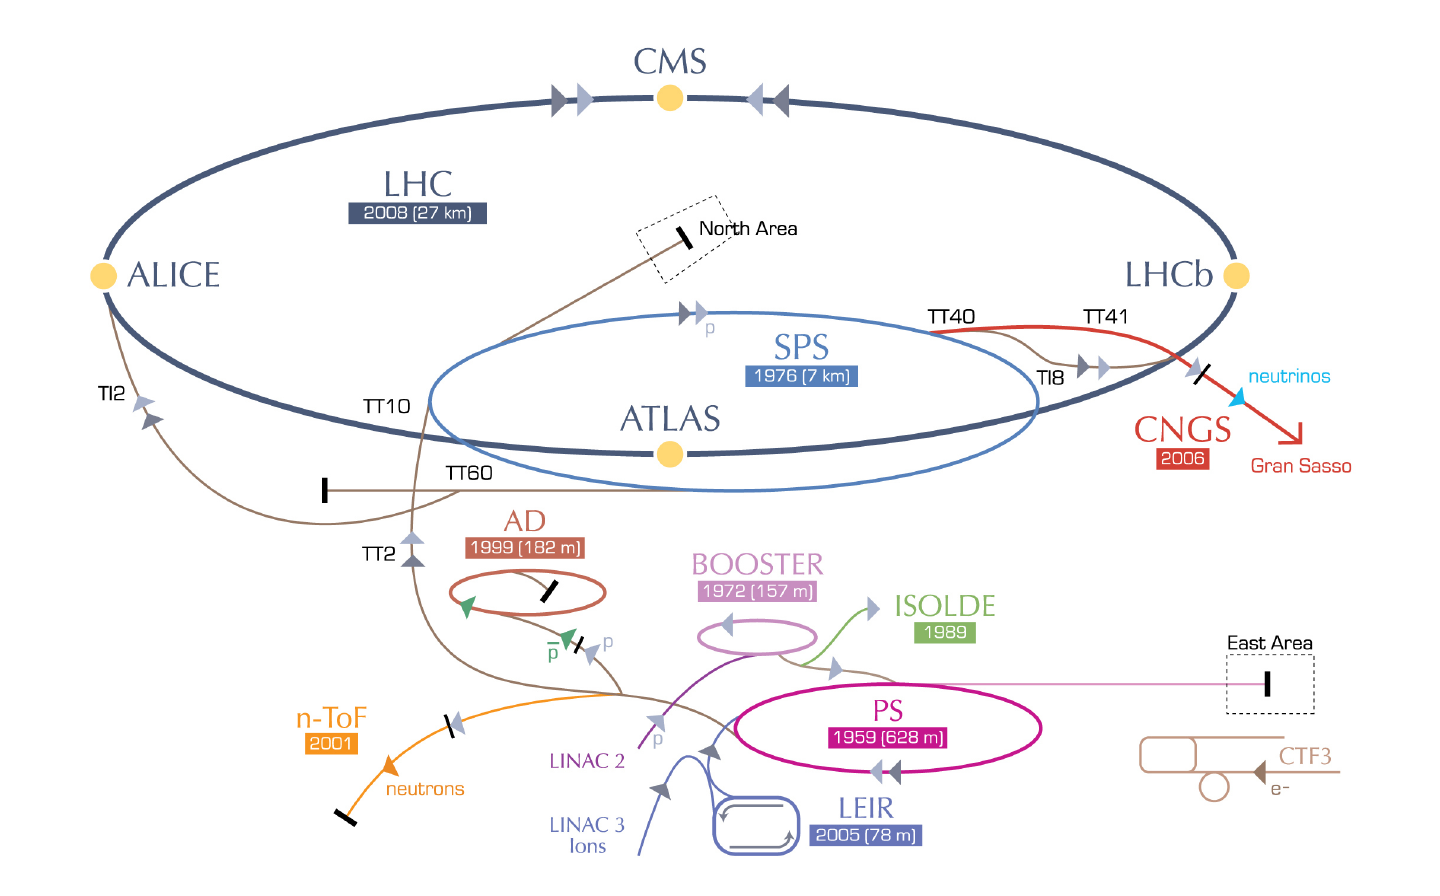
\includegraphics[width=0.79\textwidth]{figures/experiment/LHC/LHC_small.png}
  \caption{Visualisation of the LHC with its experiments and the injector chain. Taken from~\cite{bib:CERNBrochure}.}  
  \label{fig:LHC}
\end{figure}

In the LHC, the beams are kept on the circuit with the help of a magnetic field of 4.76\tesla.
Further quadrupole and sextupole magnets squeeze and focus the bunches.
They have a spread of roughly 8\cm length and a Gaussian shape radius of 20\mum RMS at the interaction point.
The number of contained protons in each bunch is of the order $10^{11}$.
The LHC has eight different insertion region, where four of them are dedicated to the four main experiments of the LHC, the CMS, ATLAS, LHCb and ALICE experiments.
The CMS~\cite{bib:CMS:experiment,bib:CMS:TDR} and ATLAS~\cite{bib:ATLAS:experiment,bib:ATLAS:TDR_1,bib:ATLAS:TDR_2} experiments are so-called ``general purpose experiments'', not designed for one specific task.
In contrary, the LHCb~\cite{bib:LHCb:experiment} and the ALICE~\cite{bib:ALICE:experiment} experiment are designed with an emphasis on CP-violation measurements and heavy ion collisions, respectively.
Each experiment is interested thus in different processes to happen at the beam collision points.
The number of expected event for a given process can be expressed in terms of the corresponding cross section $\sigma$ times the integrated luminosity.
\begin{equation}
N = L \cdot \sigma,
\end{equation}
with an integrated luminosity of $L=\int \mathcal{L}\, dt$, where $\mathcal{L}$ is the instantaneous luminosity (which can change over time).

The instantaneous luminosity $\mathcal{L}$ depends on the several machine parameters, such as the collision frequency $f$, the number of particles in the bunches $n_1$ and $n_2$,
the spread in the transverse plane of the bunches $\sigma_x$ and $\sigma_y$ and a geometrical correction parameter $F$ due to the crossing angle of the two bunches at the interaction point
\begin{equation}
\mathcal{L} = \frac{f n_1 n_2 }{4 \pi \sigma_x \sigma_y} \cdot F.
\end{equation}
In 2012, the peak luminosity was $7.7 \cdot 10^{33} \frac{1}{\text{cm}^2\,\text{s}}$.
The total integrated luminosity over time recorded at the CMS experiment is shown in Fig.~\ref{fig:Lumi}.

\begin{figure}[!b]
  \centering
      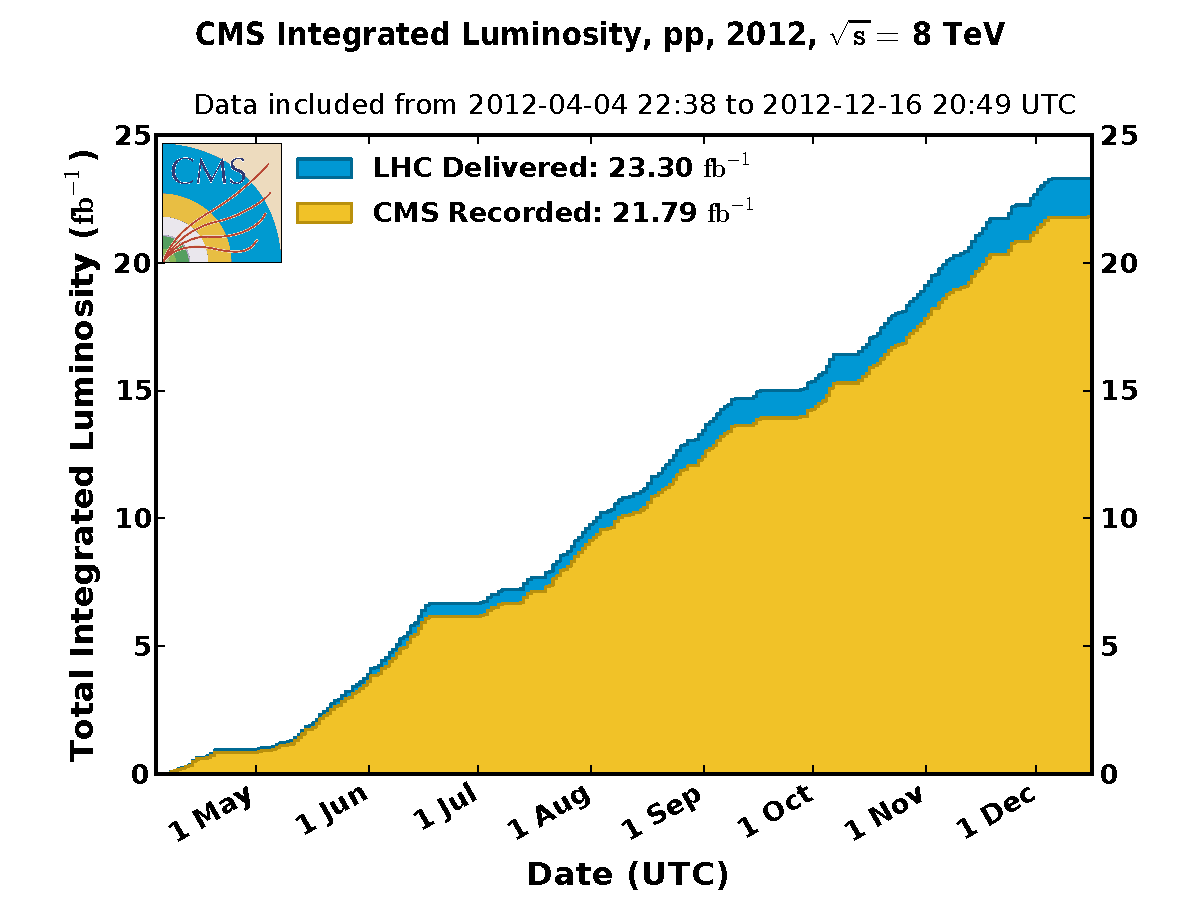
\includegraphics[width=0.59\textwidth]{figures/experiment/LHC/int_lumi_per_day_cumulative_pp_2012.pdf}
  \caption{Integrated luminosity delivered by LHC (blue) and recorded by CMS (orange) in the year 2012. Taken from~\cite{bib:LumiWiki}.}  
  \label{fig:Lumi}
\end{figure}

%%%%%%%%%%%%%%%%%%%%%%%%%%%%%%%%%%%%%%%%%%%%%%%%%%%%%%%%%%%%%%%%%%%%%%%%%%%%%%%%%%%%%%%%%%%%%%%%%%%%%%%%%%%%%%%%%%%%%%%%%%%%%%%%%%%%%%%%%%%%%%%%%%%%%%%%%%%%%%%%%%%%%%%%%%%%%%%%%%%%%%%%%%%%%%%%%%%%%%%%%%%%%%%%%%%%%%%%%%%%%%%%%%%
%%%%%%%%%%%%%%%%%%%%%%%%%%%%%%%%%%%%%%%%%%%%%%%%%%%%%%%%%%%%%%%%%%%%%%%%%%%%%%%%%%%%%%%%%%%%%%%%%%%%%%%%%%%%%%%%%%%%%%%%%%%%%%%%%%%%%%%%%%%%%%%%%%%%%%%%%%%%%%%%%%%%%%%%%%%%%%%%%%%%%%%%%%%%%%%%%%%%%%%%%%%%%%%%%%%%%%%%%%%%%%%%%%%
%%%%%%%%%%%%%%%%%%%%%%%%%%%%%%%%%%%%%%%%%%%%%%%%%%%%%%%%%%%%%%%%%%%%%%%%%%%%%%%%%%%%%%%%%%%%%%%%%%%%%%%%%%%%%%%%%%%%%%%%%%%%%%%%%%%%%%%%%%%%%%%%%%%%%%%%%%%%%%%%%%%%%%%%%%%%%%%%%%%%%%%%%%%%%%%%%%%%%%%%%%%%%%%%%%%%%%%%%%%%%%%%%%%
\FloatBarrier
\chapter{The CMS detector}
The Compact Muon Solenoid (CMS) detector~\cite{bib:CMS:experiment,bib:CMS:TDR} is a general purpose detector, designed to explore particle physics phenomena up to the multi-TeV scale.
The detector concept is an onion-like structure of different layers, each one made up with a different type of detector. 
The CMS detector measures 21.6\m in length and 14.6\m in diameter with a total weight of 12500\,tons.
In Fig.~\ref{fig:CMSdetector}, a perspective view of the CMS detector is depicted. 
\begin{figure}[!b]
  \centering
      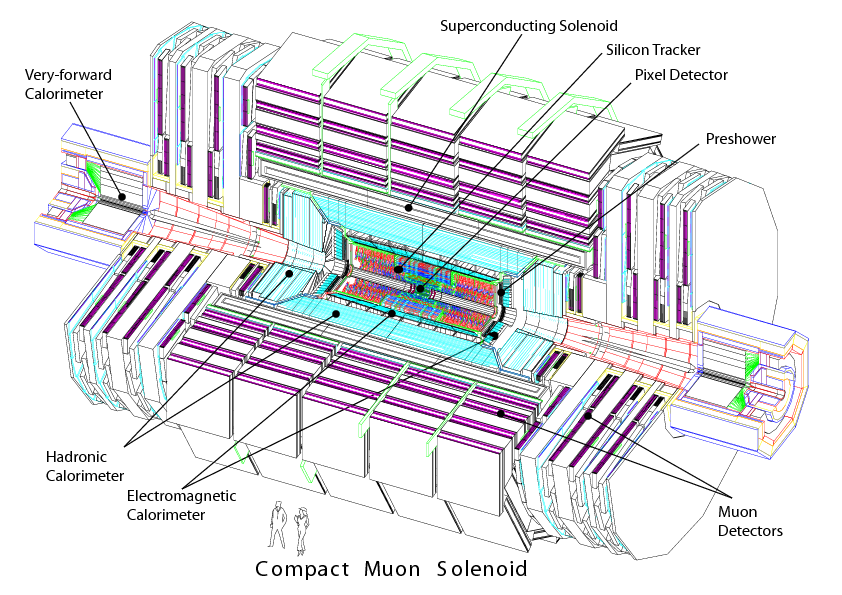
\includegraphics[width=0.99\textwidth]{figures/experiment/CMS/cms_complete_labelled.png}
  \caption{A perspective view of the CMS detector. Taken from~\cite{bib:CMS:experiment}}  
  \label{fig:CMSdetector}
\end{figure}

The used coordinate system at the CMS experiment consists of the pseudorapidity $\eta = -\ln \tan{\frac{\theta}{2}}$ and the azimuthal angle $\phi$.
The advantage of the pseudorapidity $\eta$ is the Lorentz invariance with respect to the z-axis (beam axis).
The angle $\phi$ covers the direction in the $x-y$ plane (orthogonal to the beam axis).

In order to measure the momentum of charged particles a superconducting solenoid is incorporated between the calorimeter system and the muon system providing a uniform axial magnet field of 3.8\tesla.
Incorporated iron yokes contained within the muon system ensure the return of the magnetic flux. 

In the following, the various detector components of the CMS detector from the inside to the outside as well as the trigger system will be explained.
%%%%%%%%%%%%%%%%%%%%%%%%%%%%%%%%%%%%%%%%%%%%%%%%%%%%%%%%%%%%%%%%%%%%%%%%%%%%%%%%%%%%%%%%%%%%%%%%%%%%%%%%%%%%%%%%%%%%%%%%%%%%%%%%%%%%%%%%%%%%%%%%%%%%%%%%%%%%%%%%%%%%%%%%%%%%%%%%%%%%%%%%%%%%%%%%%%%%%%%%%%%%%%%%%%%%%%%%%%%%%%%%%%%
\FloatBarrier
\section{The tracking system}
The tracking detector~\cite{bib:CMS:Tracker_1997,bib:CMS:Tracker_2000} is the innermost detector of the CMS experiment. 
It is a silicon semiconductor detector and is included for the tasks of vertex and track reconstruction by the measurement of particles' energy losses.
A schematic sketch of the tracker at CMS is depicted in Fig.~\ref{fig:Tracker}.
\begin{figure}[!b]
  \centering
      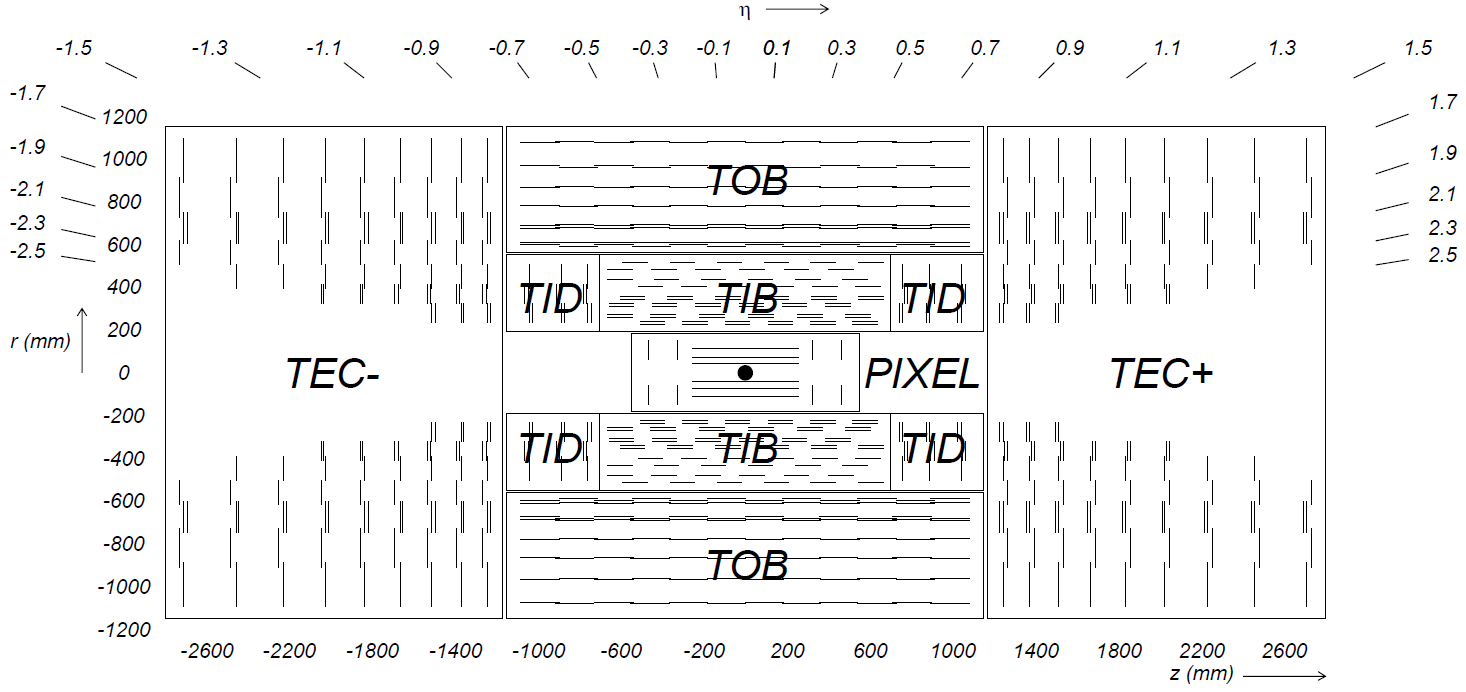
\includegraphics[width=0.99\textwidth]{figures/experiment/CMS/Figures_Experimental_Apparatus_Tracker.png}
  \caption{Schematic sketch of the silicon tracker at CMS in the $z - \phi$ plane. Taken from~\cite{bib:CMS:tracking_8TeV}.}  
  \label{fig:Tracker}
\end{figure}
The tracking system is divided into two parts, the innermost tracker is a silicon pixel detector surrounded by a silicon strip detector.
Both parts will be explained in detail in the upcoming sections, followed by a short description how the energy of a traversing particle is measured with the silicon sensors.
As a calibration of the silicon pixel detector was performed within this PhD thesis (see Section~\ref{sec:EnergyCalibration}), an emphasis will be put on the pixel detector.


%%%%%%%%%%%%%%%%%%%%%%%%%%%%%%%%%%%%%%%%%%%%%%%%%%%%%%%%%%%%%%%%%%%%%%%%%%%%%%%%%%%%%%%%%%%%%%%%%%%%%%%%%%%%%%%%%%%%%%%%%%%%%%%%%%%%%%%%%%%%%%%%%%%%%%%%%%%%%%%%%%%%%%%%%%%%%%%%%%%%%%%%%%%%%%%%%%%%%%%%%%%%%%%%%%%%%%%%%%%%%%%%%%%
\subsection*{The silicon pixel tracker}
The silicon pixel detector consists of three different cylindrical layers in the barrel region at radii of 4.4\cm, 7.3\cm and 10.2\cm and two discs in the endcaps at $z$-distances of 34.5\cm and 46.5\cm (cf. Fig.~\ref{fig:Tracker}).
It is made up of 1440 modules in total (barrel + endcaps), each module comprising 8 or 16 read-out-chips (ROCs).
The read-out-chips are bump bonded~\cite{Thesis_Jenny} to a pixel system of $52\times80$ pixels, which are read out in double columns (see~\cite{Thesis_Jenny} on detailed information of the readout electronics).
A visualisation of a part of a pixel module is shown in Fig.~\ref{fig:PixelTracker}.
\begin{figure}[!b]
  \centering
      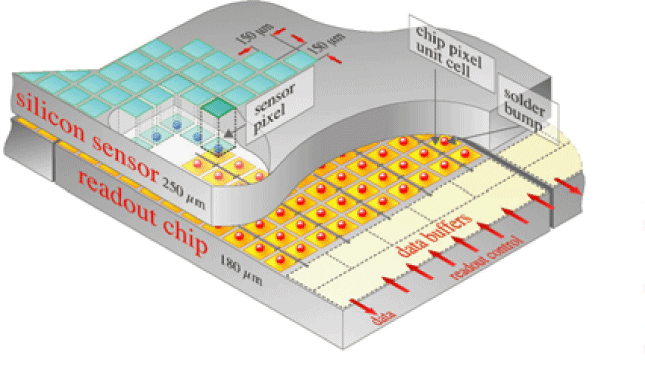
\includegraphics[width=0.99\textwidth]{figures/experiment/CMS/Pixelement.png}
  \caption{Schematic sketch of a part of a silicon pixel tracker module including the silicon sensors and the read-out-chip (ROC). Taken from~\cite{bib:CMS:tracking_8TeV}.}  
  \label{fig:PixelTracker}
\end{figure}
In total, there 65 million pixels comprised in the pixel detector.
The large number of pixels and their small size ensure a low occupancy close to the vertex of around $0.002 - 0.02$\%~\cite{bib:CMS:tracking_8TeV} and a high hit efficiency of around 99\%~\cite{bib:CMS:PixelSpatialResolution}. 

The silicon pixel detector is very important for the reconstruction of primary and secondary vertices as well as the reconstruction of particle tracks.
Therefore a high spatial resolution is needed.
This is achieved by the small size of the pixels ($ 150 \times 100 \mum^2$) and the exploitation of the spread of the energy deposition across several pixels (in average the energy is deposited across 3-5 pixels~\cite{bib:TWIKI:PixelClusterSize}).
Exploiting the energy spread across pixels, a spatial resolution in the barrel region of 9.4\mum in the $r - \phi$ plane and - dependent on the incident angle of a track - a hit resolution between $20-45\mum$ in the z-direction is achieved~\cite{bib:CMS:tracking_8TeV}. 
The high spatial resolution makes the pixel detector perfectly suited for the reconstruction of vertices and tracks.
The spatial resolution of the primary vertex depends on the number of tracks taken into account for the reconstruction of the primary vertex.
For more than 50 tracks originating from the primary vertex the spatial resolution is around $10-12\mum$ for each of the three spatial dimensions~\cite{bib:CMS:tracking_8TeV}.
The reconstruction efficiency of primary vertices is close to 100\% for more than two tracks used for the vertex reconstruction~\cite{bib:CMS:tracking_8TeV}.

%The momentum resolution of the full tracking system will be discussed in Section~\ref{FIXME}.

\subsection*{The silicon strip tracker}
The silicon strip tracker is the next-to innermost detector of the CMS experiment and ranges up to a radius of 116\cm.
The barrel region consists of a tracker inner barrel (TIB) and a tracker outer barrel (TOB).
The TIB has four layers (2 layers with stereo modules to measure the hit position additionally in the $r-z$ plane) with silicon sensors of 320\mum thickness.
The TOB has six different layers (2 layers with stereo modules) with silicon sensors of 500\mum thickness. 

The endcaps are subdivided into a tracker endcap (TEC) and a tracker inner disk (TID).
They ensure a coverage of the up to a pseudorapidity of $|\eta|=2.5$.
In each TEC, 9 disks between a z-position of $120\cm < z < 280\cm$ are contained.
Each of the TID comprises three disks between $65\cm < z < 120\cm$.


\subsection*{Energy measurements in the tracking system}
A charged particle traversing the above mentioned silicon detectors produce electron-hole pairs in the semiconducting material along its trajectory and thus loose energy due to ionisation.
For silicon, the mean energy to create an electron-hole pair is 3.61\ev at $-10\degree$C.
Minimally ionising particles produce in average about 22000 electron-hole pairs in silicon sensors~\cite{Thesis_Jenny}.
For electrons that undergo a hard collision with the incoming particle (so-called delta-rays), produce further ionisation and can thus lead to much higher energy deposits in the silicon.
Because of the applied bias voltage at the sensors (for the creation of a depletion zone), the released electrons (holes) travel to the n-contacts (p-contacts) and induce thereby a current which is measured by the readout electronics. 
A more detailed description of the energy measurement in silicon sensors can be found in~\cite{Thesis_Jenny}.

%%%%%%%%%%%%%%%%%%%%%%%%%%%%%%%%%%%%%%%%%%%%%%%%%%%%%%%%%%%%%%%%%%%%%%%%%%%%%%%%%%%%%%%%%%%%%%%%%%%%%%%%%%%%%%%%%%%%%%%%%%%%%%%%%%%%%%%%%%%%%%%%%%%%%%%%%%%%%%%%%%%%%%%%%%%%%%%%%%%%%%%%%%%%%%%%%%%%%%%%%%%%%%%%%%%%%%%%%%%%%%%%%%%
\section{The electromagnetic calorimeter}
The electromagnetic calorimeter (ECAL)~\cite{bib:CMS:TDR_2006,bib:CMS:TDR_ECAL} encloses the tracking system and starts at a radius of 129\cm in the barrel region.
It is divided into a barrel part and two endcaps, which are at a distance of 314\cm from the vertex.
Figure~\ref{fig:ECAL} depicts a schematic sketch of the electromagnetic calorimeter system in the transverse plane.
\begin{figure}[!h]
  \centering
      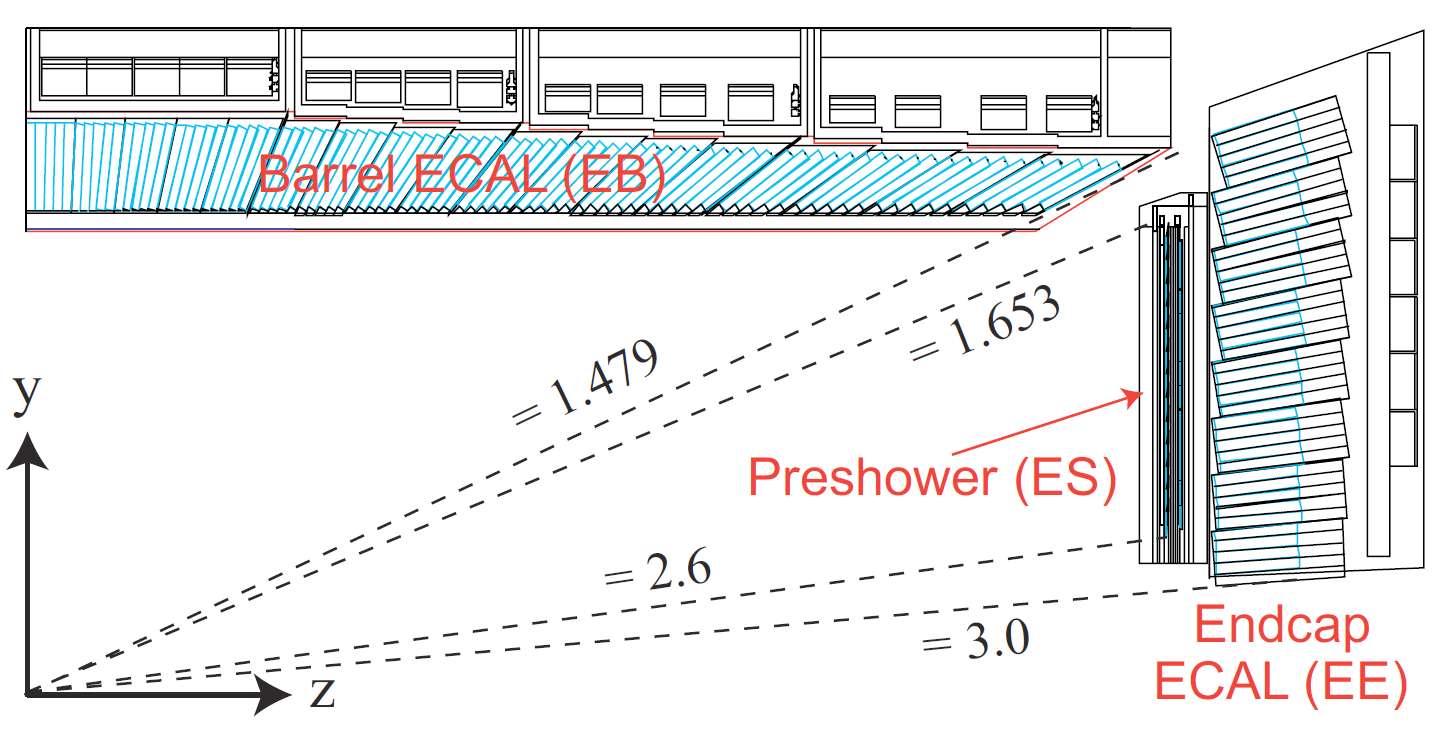
\includegraphics[width=0.89\textwidth]{figures/experiment/CMS/Figures_Experimental_Apparatus_ECALRapidity.png}
  \caption{A quarter section of the ECAL in a transverse view. Taken from~\cite{bib:CMS:TDR_2006}.}  
  \label{fig:ECAL}
\end{figure}
It can be seen, that the ECAL barrel~(EB) covers a pseudorapidity region up to $|\eta|=1.479$.
The ECAL endcaps~(EE) start at $|\eta|=1.653$ and reach up to $|\eta|=3.0$.
Before the endcaps, a preshower detector ($1.653<|\eta|<2.6$) is installed with the main task to identify neutral pions in the endcaps.
It improves additionally the position measurement of electrons and photons.

The EB and EE consist of lead tungstate (PbWO$_4$) scintillating crystals, 61200 in the barrel region and 7324 in the endcaps. 
Their advantage is the short radiation (X$_0$=0.89\cm) and Moli\`ere (2.2\cm) lengths.
Thus particles deposit on rather short distances their energy and a compact design is possible.
To detect the rather low light yield (30$\gamma$/\mev) of a traversing particle, silicon avalanche photodiodes (APDs) are used in the barrel region and vacuum  phototriodes (VPTs) in the endcaps.
For information on the readout electronics, the reader is referred to~\cite{bib:CMS:TDR_2006}.

The resolution of an energy measurement in the calorimeter can be expressed by 
\begin{equation}
\label{eq:CaloResolution}
\left( \frac{\sigma}{E} \right)^2 = \left( \frac{S}{\sqrt{E}} \right)^2 + \left( \frac{N}{E} \right)^2 +C^2,
\end{equation}
with $S$ referring to the stochastic term, $N$ to the noise term, and $C$ to a constant term.
For the ECAL the parameters of Eq.~\eqref{eq:CaloResolution} are measured to $S=3.63\sqrt{\text{GeV}}$, $N=0.124\gev$, and $C=0.26$~\cite{bib:CMS:TDR_2006}. These number lead to an energy resolution of around 0.4\% for an electron with $E \approx 200\gev$ and around 0.6\% for an electron with $E \approx 50\gev$.

%%%%%%%%%%%%%%%%%%%%%%%%%%%%%%%%%%%%%%%%%%%%%%%%%%%%%%%%%%%%%%%%%%%%%%%%%%%%%%%%%%%%%%%%%%%%%%%%%%%%%%%%%%%%%%%%%%%%%%%%%%%%%%%%%%%%%%%%%%%%%%%%%%%%%%%%%%%%%%%%%%%%%%%%%%%%%%%%%%%%%%%%%%%%%%%%%%%%%%%%%%%%%%%%%%%%%%%%%%%%%%%%%%
\section{The hadronic calorimeter}
The hadronic calorimeter (HCAL)~\cite{bib:CMS:TDR_2006,bib:CMS:TDR_HCAL} of the CMS experiment is splitted into four different detector modules: the hadron barrel (HB), the hadron outer (HO), the hadron endcap (HE) and the hadron forward (HF).
A schematic sketch is depicted in Fig.~\ref{fig:HCAL}.
\begin{figure}[!h]
  \centering
      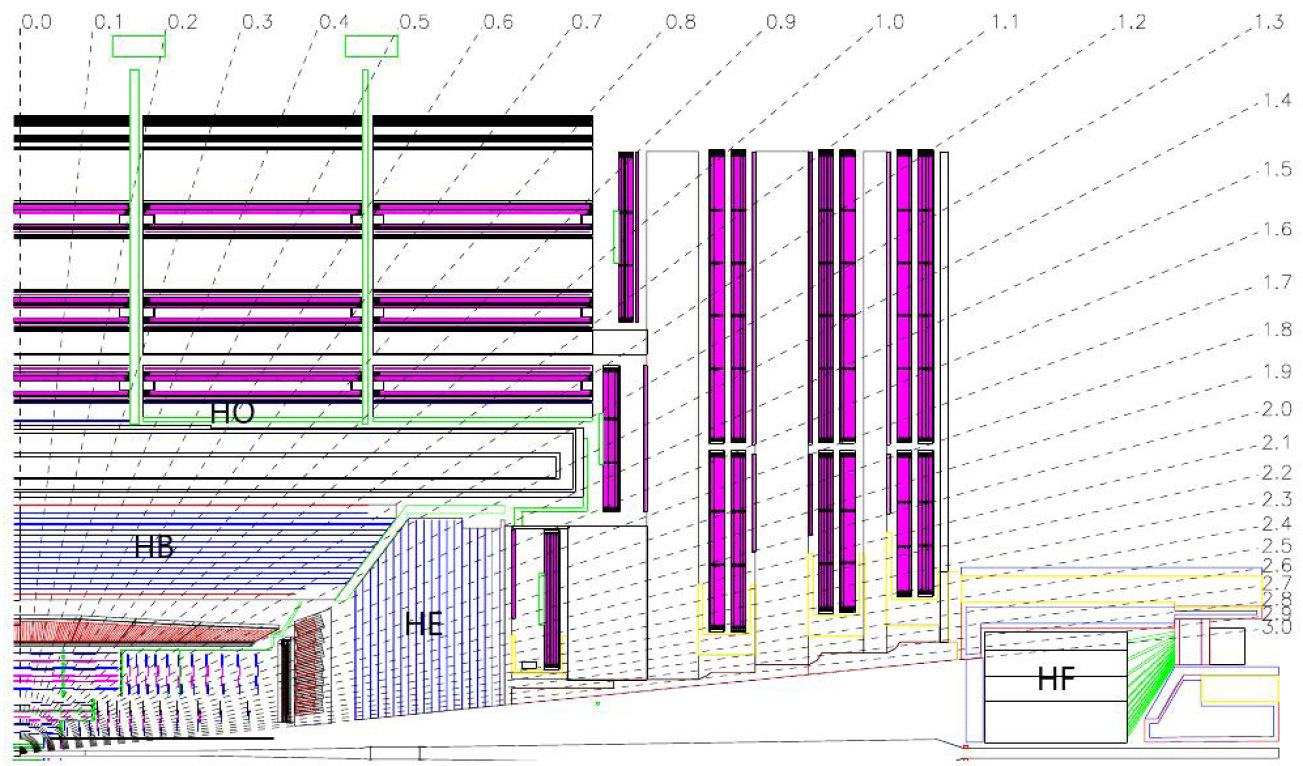
\includegraphics[width=0.79\textwidth]{figures/experiment/CMS/fig_HCALdiagram.png}
  \caption{A quarter section of the HCAL in a transverse view. Taken from~\cite{bib:CMS:HCAL_Performance_2009}.}  
  \label{fig:HCAL}
\end{figure}

The HCAL is dedicated to measure the energy of hadrons as well as providing a good estimate of the missing energy in the event.
The latter one is achieved by the high pseudorapidity coverage ($|\eta|<5.0$) in order to detect most of the visible particles.

The HCAL is a so-called sampling calorimeter which consists of brass absorber material, initiating the hadronic shower, as well as active plastic scintillators.
The emitted photons are detected with wavelength-shifting (WLS) fibres that are embedded into the scintillators.

The hadron barrel (HB) covers the pseudorapidity range between $-1.4 < \eta < 1.4$.
It is composed of 17 layers of absorber material (15 brass and 2 steal layers) interleaved with scintillator layers.
The scintillator tiles are divided into 2304 cells with a size of $\Delta \eta \times \Delta \phi = 0.087 \times 0.087$.
A group of 72 cells form a HCAL tower, which is read out with wavelength-shifting fibres.

The hadron outer (HO) covers a pseudorapidity range up to $|\eta|=1.26$ and is divided into sectors which match the $\phi$ segmentation of the drift-tube chambers of the muon system (see Section~\ref{sec:MuonSystem}).
It is located between the solenoid and the barrel detector of the muon system.
The HO is dedicated to measure the energy of the shower leakage of hadrons.
Its thickness corresponds to over ten interaction lengths.

The hadron endcap (HE) extends the pseudorapidity coverage of the HCAL up to $|\eta|=3.0$ and starts at $|\eta|=1.3$.
It consists of 2304 cells in total, which vary in size over the covered pseudorapidity range.

Finally, the hadron forward (HF) calorimeter extends the pseudorapidity range up to $|\eta|=5.0$, starting from $|\eta|=3.0$.
It is build out of steal plates, which contain 1\mm square grooves containing quartz fibres.
The emitted light by the quartz fibres is transferred to photomultipliers.
The HF is divided into a number of 13 towers where almost all towers have a spread of $\Delta \eta \approx 0.175$ in $\eta$ direction and $\sim 10\degree$ in $\phi$ direction.
 
%%%%%%%%%%%%%%%%%%%%%%%%%%%%%%%%%%%%%%%%%%%%%%%%%%%%%%%%%%%%%%%%%%%%%%%%%%%%%%%%%%%%%%%%%%%%%%%%%%%%%%%%%%%%%%%%%%%%%%%%%%%%%%%%%%%%%%%%%%%%%%%%%%%%%%%%%%%%%%%%%%%%%%%%%%%%%%%%%%%%%%%%%%%%%%%%%%%%%%%%%%%%%%%%%%%%%%%%%%%%%%%%%%
\section{The muon system}
\label{sec:MuonSystem}
The muon system~\cite{bib:CMS:TDR_2006,bib:CMS:TDR_MuonSystem} is the outermost detector component at CMS.
It comprises three different types of gaseous detectors, mounted into the iron return yokes: drift tube (DT) chambers in the barrel region ($|\eta|<1.2$), cathode strip chambers (CSC) in the endcap region ($1.04<|\eta|<2.4$) and resistive plate chambers (RPC) in the barrel as well as the endcap region ($|\eta|<1.6$) (see Fig.~\ref{fig:MuonSystem} for a schematic sketch of the muon system).
\begin{figure}[!b]
  \centering
      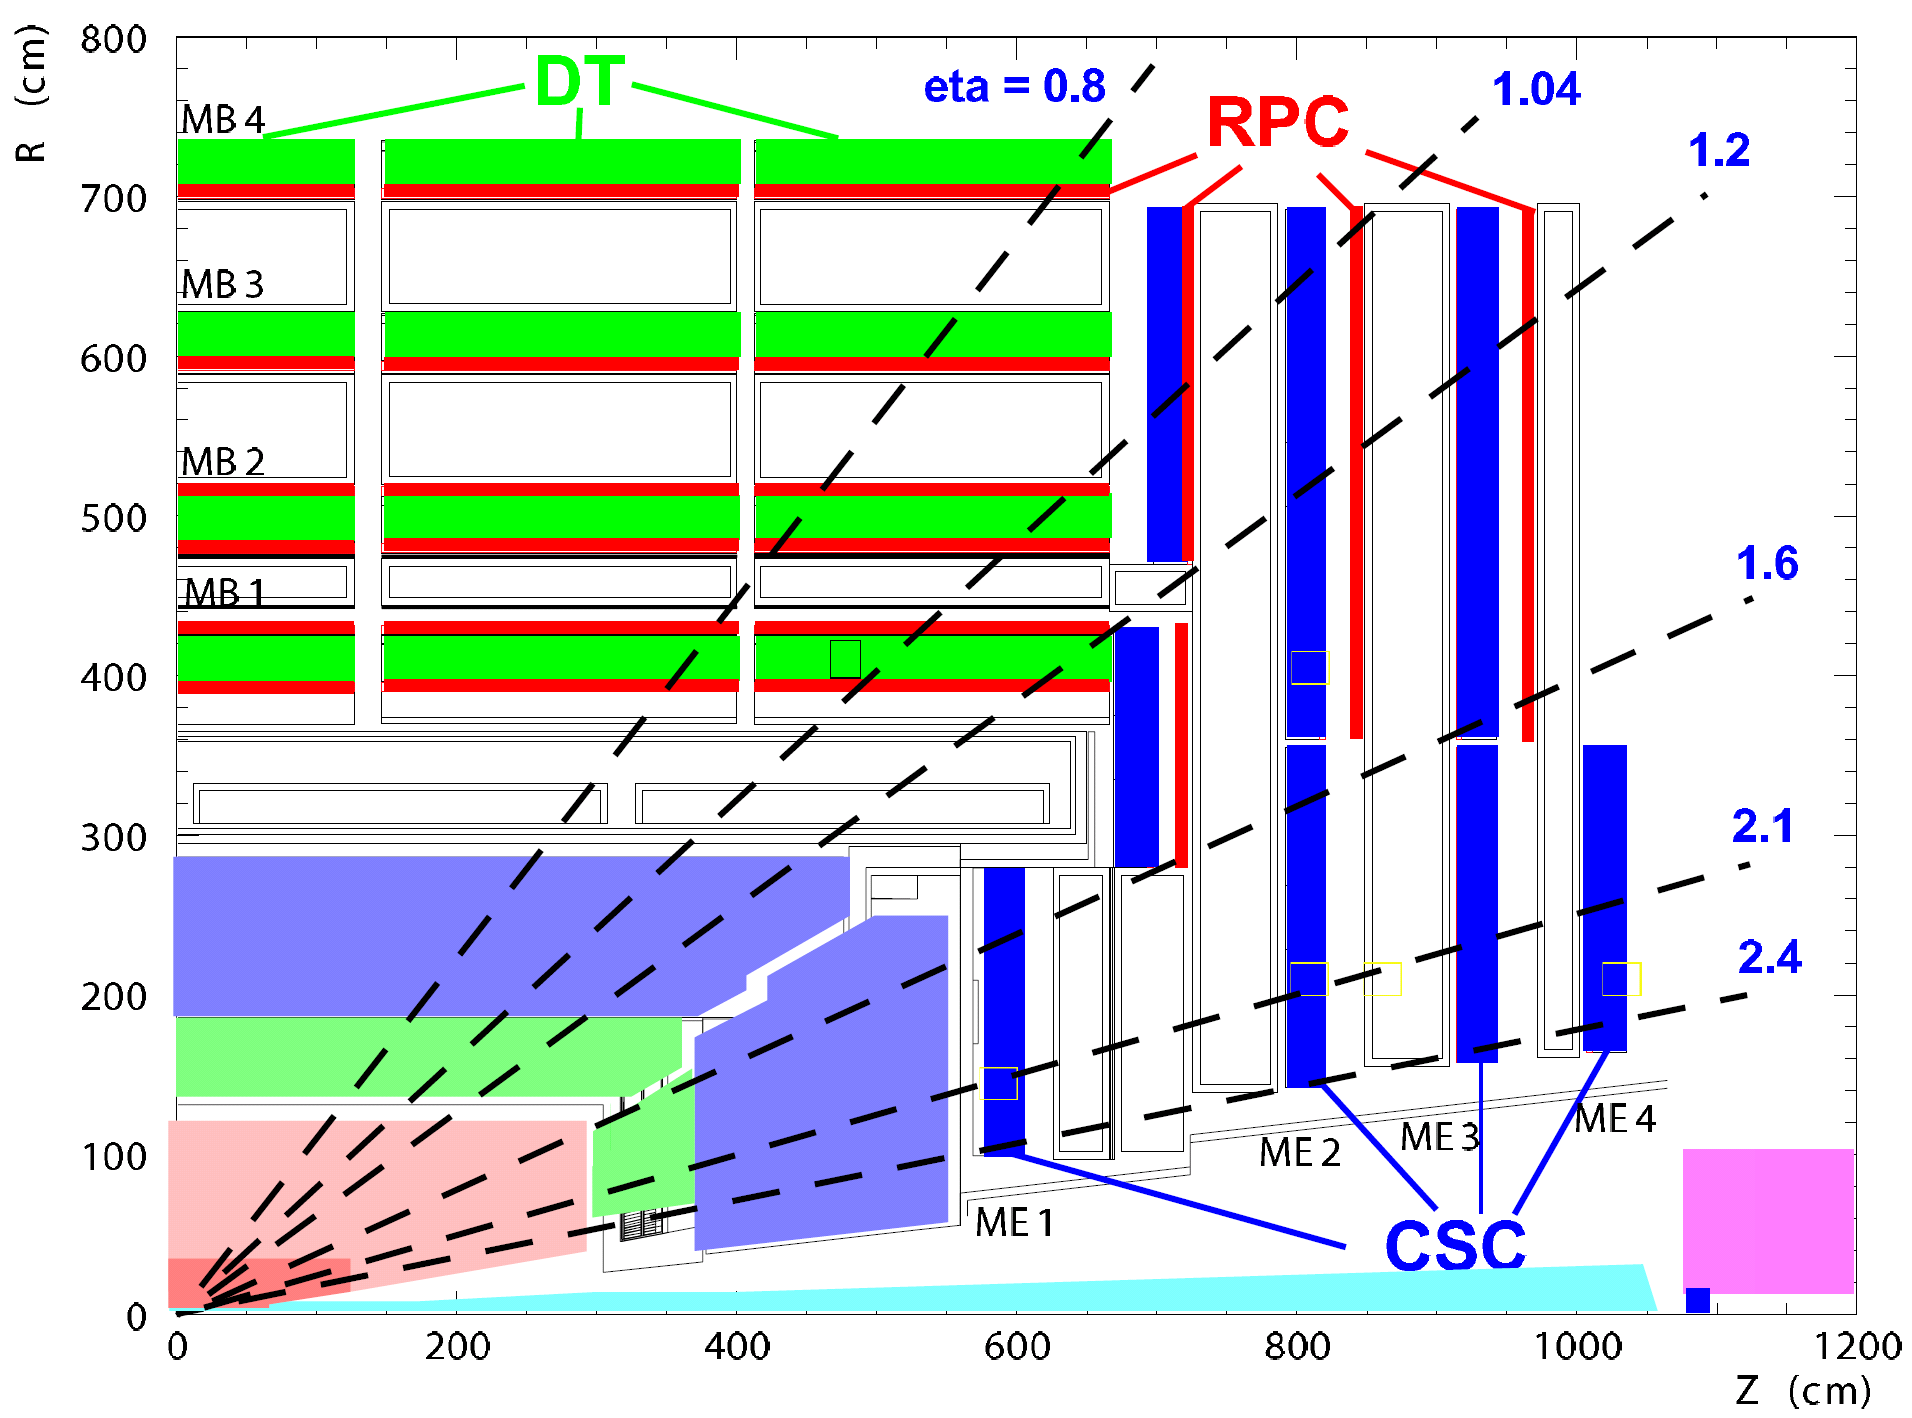
\includegraphics[width=0.69\textwidth]{figures/experiment/CMS/Figures_Experimental_Apparatus_MuonDetector.png}
  \caption{A quarter section of the CMS detector in the transverse plane with a detailed view on the muon system. Taken from~\cite{bib:CMS:TDR_2006}.}  
  \label{fig:MuonSystem}
\end{figure}
In the barrel part of the muon system four layers (so-called stations) of drift-tube chambers are assembled inside the iron return yoke layers at radii of 4.0, 4.9, 5.9 and 7.0\m from the beam axis.
The position of the muon traversing these layers can be measured with a precision of $\approx 100\mum$ in radial direction and $\approx 1\,$mrad in $\phi$ direction. 

The four endcap disks are made up of 468 cathode strip chambers in total.
By measuring the centre-of-gravity, they achieve a spatial resolution of $\approx 100-200\mum$ and an angular resolution of $\approx 10\,$mrad in $\phi$ direction.
They are designed in order to cope with a high particle flux of about 1kHz/cm$^2$ and a non-uniform magnetic field.
As signals can be transferred very fast, they are used for the level-1 trigger system.

Finally, the resistive plate chambers cover the barrel as well as the endcap region up to a pseudorapidity of $\eta=1.6$. 
They provide a fast response with a good time resolution enabling the exact identification of the bunch-crossing a muon arose from.
It is used for the level-1 trigger system as well.
%%%%%%%%%%%%%%%%%%%%%%%%%%%%%%%%%%%%%%%%%%%%%%%%%%%%%%%%%%%%%%%%%%%%%%%%%%%%%%%%%%%%%%%%%%%%%%%%%%%%%%%%%%%%%%%%%%%%%%%%%%%%%%%%%%%%%%%%%%%%%%%%%%%%%%%%%%%%%%%%%%%%%%%%%%%%%%%%%%%%%%%%%%%%%%%%%%%%%%%%%%%%%%%%%%%%%%%%%%%%%%%%%%
\section{The trigger system}
Because of the impossibility of storing each event occurring at the CMS experiment, a multistage trigger system~\cite{bib:CMS:TDR_2006} is used to achieve a drastic reduction of nearly six orders of magnitude of recorded events.
It comprises two main parts: a so-called level-1 (L1) trigger system and a high-level trigger (HLT) system.

The L1 triggers need to provide a very fast decision (3.2\mus, where around 1\mus is allocated to the actual L1 trigger calculations) whether an event shall be recorded or not.
During this time, the recorded event data is held in buffers located close to the single detector components.
Information from the muon system and the calorimeters is used for the L1-trigger decisions.
Objects used for these decisions are so-called ``trigger primitive'' objects (photons, electrons, muons, jets above certain \et and \pt thresholds and global variables like missing transverse energy, \met). 
The design value of the number of events per second that pass this trigger stage is 100\khz.

After a time of 3.2\mus, the stored data in the buffers close to the single detector components are transferred to the front-end readout buffers in case the event passed the L1-trigger requirements.
By partial event reconstruction and the use of various trigger levels (calorimeter, muon information followed by pixel information and full event reconstruction), higher event objects can be used to check whether HLT-trigger requirements are fulfilled.
On HLT level, the decision time amounts to 50\ms and a reduction from 100\khz to 100\hz of event recording is achieved.

%%%%%%%%%%%%%%%%%%%%%%%%%%%%%%%%%%%%%%%%%%%%%%%%%%%%%%%%%%%%%%%%%%%%%%%%%%%%%%%%%%%%%%%%%%%%%%%%%%%%%%%%%%%%%%%%%%%%%%%%%%%%%%%%%%%%%%%%%%%%%%%%%%%%%%%%%%%%%%%%%%%%%%%%%%%%%%%%%%%%%%%%%%%%%%%%%%%%%%%%%%%%%%%%%%%%%%%%%%%%%%%%%%%
%%%%%%%%%%%%%%%%%%%%%%%%%%%%%%%%%%%%%%%%%%%%%%%%%%%%%%%%%%%%%%%%%%%%%%%%%%%%%%%%%%%%%%%%%%%%%%%%%%%%%%%%%%%%%%%%%%%%%%%%%%%%%%%%%%%%%%%%%%%%%%%%%%%%%%%%%%%%%%%%%%%%%%%%%%%%%%%%%%%%%%%%%%%%%%%%%%%%%%%%%%%%%%%%%%%%%%%%%%%%%%%%%%%
%%%%%%%%%%%%%%%%%%%%%%%%%%%%%%%%%%%%%%%%%%%%%%%%%%%%%%%%%%%%%%%%%%%%%%%%%%%%%%%%%%%%%%%%%%%%%%%%%%%%%%%%%%%%%%%%%%%%%%%%%%%%%%%%%%%%%%%%%%%%%%%%%%%%%%%%%%%%%%%%%%%%%%%%%%%%%%%%%%%%%%%%%%%%%%%%%%%%%%%%%%%%%%%%%%%%%%%%%%%%%%%%%%%
\FloatBarrier
\chapter{Event reconstruction and particle identification}
12 pages
\section{PF algorithm}
2 pages
\section{Object reconstruction}
\subsection*{Reconstruction of tracks}
\subsection*{Reconstruction of jets}
\subsection*{Reconstruction of muons}
\subsection*{Reconstruction of electrons}
\subsection*{Reconstruction of taus}
\subsection*{Reconstruction of missing transverse energy}
\section{Event cleaning}




%%%%%%%%%%%%%%%%%%%%%%%%%%%%%%%%%%%%%%%%%%%%%%%%%%%%%%%%%%%%%%%%%%%%%%%%%%%%%%%%%%%%%%%%%%%%%%%%%%%%%%%%%%%%%%%%%%%%%%%%%%%%%%%%%%%%%%%%%%%%%%%%%%%%%%%%%%%%%%%%%%%%%%%%%%%%%%%%%%%%%%%%%%%%%%%%%%%%%%%%%%%%%%%%%%%%%%%%%%%%%%%%%%%
%%%%%%%%%%%%%%%%%%%%%%%%%%%%%%%%%%%%%%%%%%%%%%%%%%%%%%%%%%%%%%%%%%%%%%%%%%%%%%%%%%%%%%%%%%%%%%%%%%%%%%%%%%%%%%%%%%%%%%%%%%%%%%%%%%%%%%%%%%%%%%%%%%%%%%%%%%%%%%%%%%%%%%%%%%%%%%%%%%%%%%%%%%%%%%%%%%%%%%%%%%%%%%%%%%%%%%%%%%%%%%%%%%%
%%%%%%%%%%%%%%%%%%%%%%%%%%%%%%%%%%%%%%%%%%%%%%%%%%%%%%%%%%%%%%%%%%%%%%%%%%%%%%%%%%%%%%%%%%%%%%%%%%%%%%%%%%%%%%%%%%%%%%%%%%%%%%%%%%%%%%%%%%%%%%%%%%%%%%%%%%%%%%%%%%%%%%%%%%%%%%%%%%%%%%%%%%%%%%%%%%%%%%%%%%%%%%%%%%%%%%%%%%%%%%%%%%%
\FloatBarrier
\chapter{Event simulation}

Needed:
\begin{itemize}
\item Some information on simulation
\item PDF !
\end{itemize}

3-4 pages
